%%%%%%%%%% NO OLVIDAR COLOCAR ESTE COMENTARIO CON EL NUMERO DE EJERCICIO %%%%%%%%%%%%%
%%%%%%%%%%%%%%%%%%% EJERCICIO 7 %%%%%%
%%Text bf para negrilla , el \\ es para el salto de linea.
%%El primer \\ hace un espacio en el texto y el 2 \\ crea otro espacio
\textbf{Ejemplo 5}\newline
El contrato de arriendo de una casa estipula pagos mensuales de 40.000 COP, al principio de cada mes durante un año. Si suponemos un interés del 30\% nominal anual mes anticipado. ¿Cuál será el valor del pago único que, hecho al principio del contrato?\\ \\

\textbf{Solución.}\\
\begin{center}

 \renewcommand{\arraystretch}{1.5}% Margenes de las celdas
 %Creación de la cuadricula
 \begin{longtable}{|c|c|c| }
  %Creamos una linea horizontal
  \hline
  %Definimos el color de la primera fila
  \rowcolor[HTML]{FFB183}
  %%%%% INICIO ASIGNACIÓN FECHA FOCAL %%%%%%%
  %%%%%%%%%% INICIO TITULO
  %Lo que se hace aquí es mezclar las 3 columnas en una sola
  \multicolumn{3}{|c|}{\cellcolor[HTML]{FFB183}\textbf{1. Asignación período focal}}                           \\ \hline
  %%%%%%%%%% FIN TITULO
  %%%%% INICIO DECLARACIÓN DE VARIABLES %%%%%%%
  \multicolumn{3}{|c|}{$pf = 0 pma$}                                                                         \\ \hline
  %Definimos el color de la primera fila
  \rowcolor[HTML]{FFB183}
  %%%%% INICIO DECLARACIÓN DE VARIABLES %%%%%%%
  %%%%%%%%%% INICIO TITULO
  \multicolumn{3}{|c|}{\cellcolor[HTML]{FFB183}\textbf{2. Declaración de variables}}                         \\ \hline
  %%%%%%%%%% FIN TITULO
  %%%%%%%%%% INICIO DE MATEMÁTICAS
  R= 40.000 COP & \multicolumn{2}{|c|}{$j=30\% nama \equiv 2.5\% pma= i $} \\ \hline
  $n=12 pma$    & \multicolumn{2}{|c|}{$VP_{a}= ? COP $}                                                          \\ \hline

  %%%%%%%%%% FIN DE MATEMÁTICAS
  %%%%% FIN DECLARACIÓN DE VARIABLES


  %%%%% INICIO FLUJO DE CAJA
  \rowcolor[HTML]{FFB183}
  \multicolumn{3}{|c|}{\cellcolor[HTML]{FFB183}\textbf{3. Diagrama de flujo de caja}}                        \\ \hline
  %Mezclamos 3 columnas y pondremos el dibujo
  %%%%%%%%%%%%% INSERCIÓN DE LA IMAGEN
  \multicolumn{3}{|c|}{ 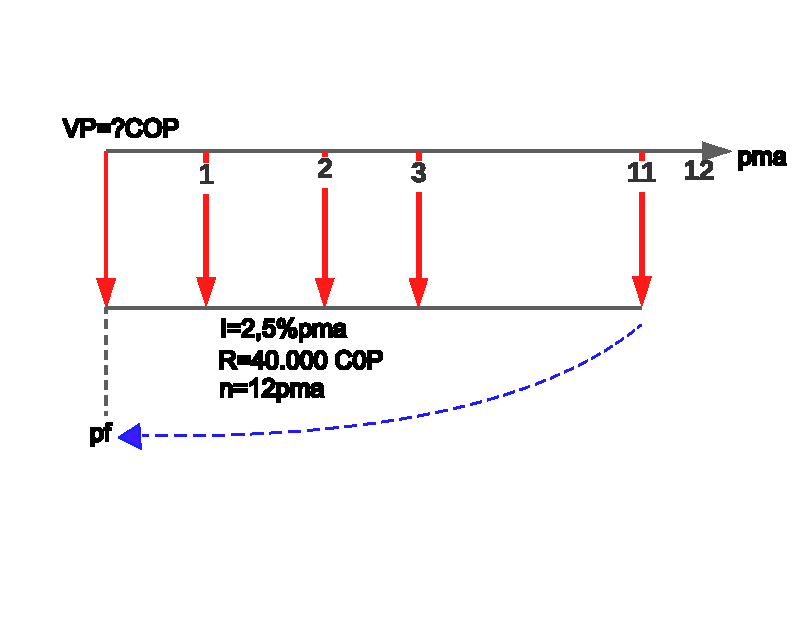
\includegraphics[width=0.90\columnwidth, trim=-5 -5 -5 -10]{4_Capitulo/img/ejemplos/6/capitulo4ejemplo6.pdf} } \\ \hline
  %%%%%%%%%%%%% FIN INSERCIÓN DE IMAGEN
  %%%%%FIN FLUJO DE CAJA



  %%%%% INICIO DECLARACIÓN FORMULAS
  %%%%%%%%%%% INICIO TITULO
  \rowcolor[HTML]{FFB183}
  \multicolumn{3}{|c|}{\cellcolor[HTML]{FFB183}\textbf{4. Declaración de fórmulas}}                          \\ \hline
  %%%%%%%%%%% FIN TITULO
  %%%%%%%%%%% INICIO MATEMÁTICAS

  \multicolumn{3}{|c|}{{$VP_{a}=R \frac{1-(1+i)^{-n}}{i} (1+i)$} \hspace{0.3cm} \textit{Valor presente serie uniforme anticipada}}    \\ \hline                                       
  \multicolumn{3}{|c|}{\cellcolor[HTML]{FFB183}\textbf{5. Desarrollo matemático}}                            \\ \hline
  %%%%%%%%%% FIN TITULO
  %%%%%%%%%% INICIO MATEMÁTICAS
  \multicolumn{3}{|c|}{$VP_{a}=$40.000 COP$\frac{1-(1+0,025)^{-12}}{0,025}(1+0,025)=$ 420.568,35 COP    }                        \\ \hline
  %%%%%%%%%% FIN MATEMÁTICAS
  %%%%%% FIN DESARROLLO MATEMÁTICO

  \rowcolor[HTML]{FFB183}
  \multicolumn{3}{|c|}{\cellcolor[HTML]{FFB183}\textbf{6. Respuesta}}                                        \\ \hline

  \multicolumn{3}{|c|}{El valor del pago unico será de 420.568 COP}                                                                \\ \hline
 \end{longtable}
 %Se crean dos lineas en blanco para que no quede el siguiente texto tan pegado
 %\newline \newline
\end{center}
%%%%%%%%%%%%%%%%%%%%%%%%%%FIN EJERCICIO 6 %%%%%%%%%%%%%%%%%%%%%%%%%%%
